\documentclass{standalone}
\usepackage{tikz}
\usetikzlibrary{patterns, positioning}
\usepackage[sfdefault]{ClearSans} %% option 'sfdefault' activates Clear Sans as the default text font
\usepackage[T1]{fontenc}

\begin{document}
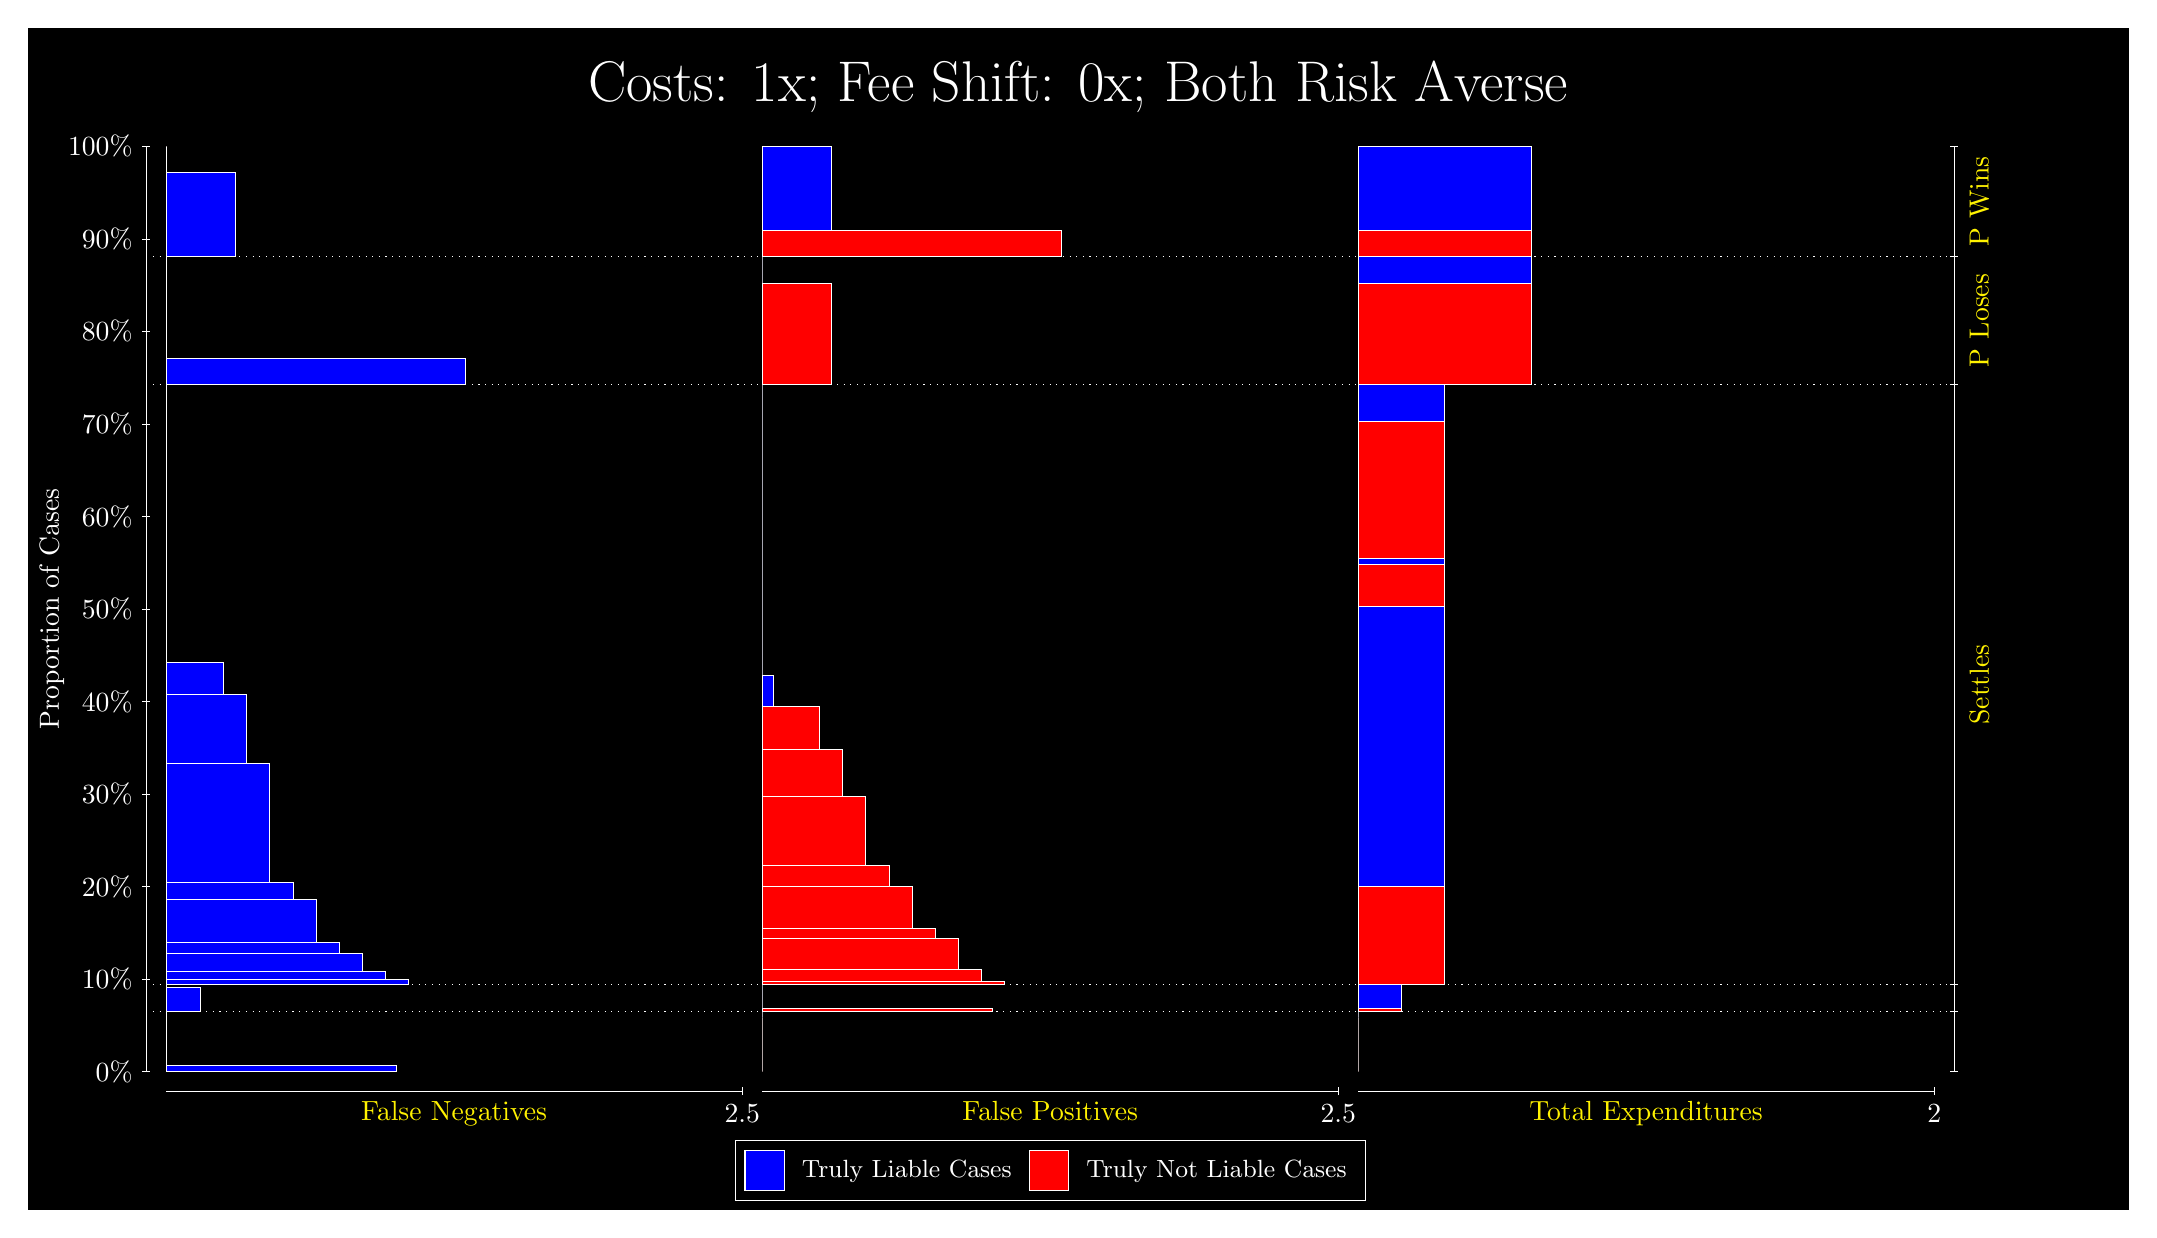
\begin{tikzpicture}
\draw[fill=black] (0,0) rectangle (26.667,15);
\draw[text=white] (0,13.5) rectangle (26.667,15) node[midway] {\huge Costs: 1x; Fee Shift: 0x; Both Risk Averse};
\draw[white, very thin] (1.5,1.75) -- (1.5,13.5);
\node[rotate=90, text=white, anchor=center] at (0.3, 7.625) {Proportion of Cases};
\draw[white, very thin] (1.45,1.75) -- (1.55,1.75);
\node[text=white, anchor=east] at (1.45, 1.75) {0\%};
\draw[white, very thin] (1.45,2.925) -- (1.55,2.925);
\node[text=white, anchor=east] at (1.45, 2.925) {10\%};
\draw[white, very thin] (1.45,4.1) -- (1.55,4.1);
\node[text=white, anchor=east] at (1.45, 4.1) {20\%};
\draw[white, very thin] (1.45,5.275) -- (1.55,5.275);
\node[text=white, anchor=east] at (1.45, 5.275) {30\%};
\draw[white, very thin] (1.45,6.45) -- (1.55,6.45);
\node[text=white, anchor=east] at (1.45, 6.45) {40\%};
\draw[white, very thin] (1.45,7.625) -- (1.55,7.625);
\node[text=white, anchor=east] at (1.45, 7.625) {50\%};
\draw[white, very thin] (1.45,8.8) -- (1.55,8.8);
\node[text=white, anchor=east] at (1.45, 8.8) {60\%};
\draw[white, very thin] (1.45,9.975) -- (1.55,9.975);
\node[text=white, anchor=east] at (1.45, 9.975) {70\%};
\draw[white, very thin] (1.45,11.15) -- (1.55,11.15);
\node[text=white, anchor=east] at (1.45, 11.15) {80\%};
\draw[white, very thin] (1.45,12.325) -- (1.55,12.325);
\node[text=white, anchor=east] at (1.45, 12.325) {90\%};
\draw[white, very thin] (1.45,13.5) -- (1.55,13.5);
\node[text=white, anchor=east] at (1.45, 13.5) {100\%};

\draw[white, very thin] (24.457,1.75) -- (24.457,13.5);
\draw[white, very thin] (24.407,1.75) -- (24.507,1.75);
\node[anchor=west] at (24.407, 1.75) {};
\draw[white, very thin] (24.407,2.5152) -- (24.507,2.5152);
\node[anchor=west] at (24.407, 2.5152) {};
\draw[white, very thin] (24.407,2.8533) -- (24.507,2.8533);
\node[anchor=west] at (24.407, 2.8533) {};
\draw[white, very thin] (24.407,10.476) -- (24.507,10.476);
\node[anchor=west] at (24.407, 10.476) {};
\draw[white, very thin] (24.407,12.101) -- (24.507,12.101);
\node[anchor=west] at (24.407, 12.101) {};
\draw[white, very thin] (24.407,13.5) -- (24.507,13.5);
\node[anchor=west] at (24.407, 13.5) {};

\draw[white, very thin, fill=blue] (1.75,1.75) rectangle (4.6775,1.8305);
\draw[white, very thin, fill=red] (1.75,1.8305) rectangle (1.75,2.5152);
\draw[white, very thin, fill=blue] (1.75,2.5152) rectangle (2.1891,2.8181);
\draw[white, very thin, fill=red] (1.75,2.8181) rectangle (1.75,2.8533);
\draw[white, very thin, fill=blue] (1.75,2.8533) rectangle (4.8239,2.9251);
\draw[white, very thin, fill=blue] (1.75,2.9251) rectangle (4.5312,3.0278);
\draw[white, very thin, fill=blue] (1.75,3.0278) rectangle (4.2384,3.2474);
\draw[white, very thin, fill=blue] (1.75,3.2474) rectangle (3.9457,3.3978);
\draw[white, very thin, fill=blue] (1.75,3.3978) rectangle (3.6529,3.9355);
\draw[white, very thin, fill=blue] (1.75,3.9355) rectangle (3.3602,4.152);
\draw[white, very thin, fill=blue] (1.75,4.152) rectangle (3.0674,5.6705);
\draw[white, very thin, fill=blue] (1.75,5.6705) rectangle (2.7746,6.5469);
\draw[white, very thin, fill=blue] (1.75,6.5469) rectangle (2.4819,6.9444);
\draw[white, very thin, fill=red] (1.75,6.9444) rectangle (1.75,10.476);
\draw[white, very thin, fill=blue] (1.75,10.476) rectangle (5.5558,10.81);
\draw[white, very thin, fill=red] (1.75,10.81) rectangle (1.75,12.101);
\draw[white, very thin, fill=blue] (1.75,12.101) rectangle (2.6283,13.167);
\draw[white, very thin, fill=red] (1.75,13.167) rectangle (1.75,13.5);
\draw[white, very thin, fill=red] (9.3189,1.75) rectangle (9.3189,2.4347);
\draw[white, very thin, fill=blue] (9.3189,2.4347) rectangle (9.3189,2.5152);
\draw[white, very thin, fill=red] (9.3189,2.5152) rectangle (12.246,2.5504);
\draw[white, very thin, fill=blue] (9.3189,2.5504) rectangle (9.3189,2.8533);
\draw[white, very thin, fill=red] (9.3189,2.8533) rectangle (12.393,2.8975);
\draw[white, very thin, fill=red] (9.3189,2.8975) rectangle (12.1,3.0427);
\draw[white, very thin, fill=red] (9.3189,3.0427) rectangle (11.807,3.448);
\draw[white, very thin, fill=red] (9.3189,3.448) rectangle (11.515,3.5661);
\draw[white, very thin, fill=red] (9.3189,3.5661) rectangle (11.222,4.1005);
\draw[white, very thin, fill=red] (9.3189,4.1005) rectangle (10.929,4.102);
\draw[white, very thin, fill=red] (9.3189,4.102) rectangle (10.929,4.3668);
\draw[white, very thin, fill=red] (9.3189,4.3668) rectangle (10.636,5.2511);
\draw[white, very thin, fill=red] (9.3189,5.2511) rectangle (10.344,5.8478);
\draw[white, very thin, fill=red] (9.3189,5.8478) rectangle (10.051,6.3853);
\draw[white, very thin, fill=blue] (9.3189,6.3853) rectangle (9.4652,6.7828);
\draw[white, very thin, fill=blue] (9.3189,6.7828) rectangle (9.3189,10.476);
\draw[white, very thin, fill=red] (9.3189,10.476) rectangle (10.197,11.767);
\draw[white, very thin, fill=blue] (9.3189,11.767) rectangle (9.3189,12.101);
\draw[white, very thin, fill=red] (9.3189,12.101) rectangle (13.125,12.434);
\draw[white, very thin, fill=blue] (9.3189,12.434) rectangle (10.197,13.5);
\draw[white, very thin, fill=red] (16.888,1.75) rectangle (16.888,2.4347);
\draw[white, very thin, fill=blue] (16.888,2.4347) rectangle (16.888,2.5152);
\draw[white, very thin, fill=red] (16.888,2.5152) rectangle (17.437,2.5504);
\draw[white, very thin, fill=blue] (16.888,2.5504) rectangle (17.437,2.8533);
\draw[white, very thin, fill=red] (16.888,2.8533) rectangle (17.986,4.102);
\draw[white, very thin, fill=blue] (16.888,4.102) rectangle (17.986,7.6549);
\draw[white, very thin, fill=red] (16.888,7.6549) rectangle (17.986,8.1924);
\draw[white, very thin, fill=blue] (16.888,8.1924) rectangle (17.986,8.2642);
\draw[white, very thin, fill=red] (16.888,8.2642) rectangle (17.986,10.01);
\draw[white, very thin, fill=blue] (16.888,10.01) rectangle (17.986,10.476);
\draw[white, very thin, fill=red] (16.888,10.476) rectangle (19.083,11.767);
\draw[white, very thin, fill=blue] (16.888,11.767) rectangle (19.083,12.101);
\draw[white, very thin, fill=red] (16.888,12.101) rectangle (19.083,12.434);
\draw[white, very thin, fill=blue] (16.888,12.434) rectangle (19.083,13.5);
\draw[white, dotted] (1.5,2.5152) -- (24.457,2.5152);
\draw[white, dotted] (1.5,2.8533) -- (24.457,2.8533);
\draw[white, dotted] (1.5,10.476) -- (24.457,10.476);
\draw[white, dotted] (1.5,12.101) -- (24.457,12.101);
\draw[white, very thin] (1.75,1.5) -- (9.0689,1.5);
\node[text=yellow, anchor=north] at (5.4094, 1.5) {False Negatives};
\draw[white, very thin] (9.0689,1.45) -- (9.0689,1.55);
\node[text=white, anchor=north] at (9.0689, 1.45) {2.5};

\draw[white, very thin] (9.3189,1.5) -- (16.638,1.5);
\node[text=yellow, anchor=north] at (12.978, 1.5) {False Positives};
\draw[white, very thin] (16.638,1.45) -- (16.638,1.55);
\node[text=white, anchor=north] at (16.638, 1.45) {2.5};

\draw[white, very thin] (16.888,1.5) -- (24.207,1.5);
\node[text=yellow, anchor=north] at (20.547, 1.5) {Total Expenditures};
\draw[white, very thin] (24.207,1.45) -- (24.207,1.55);
\node[text=white, anchor=north] at (24.207, 1.45) {2};



\node[text=yellow, centered, rotate=90] at (24.777, 6.6649) {Settles};
\node[text=yellow, centered, rotate=90] at (24.777, 11.288) {P Loses};
\node[text=yellow, centered, rotate=90] at (24.777, 12.8) {P Wins};

\draw (12.978300999999998,1.5) node[draw=none] (baseCoordinate) {};
\begin{scope}[align=center]
        \matrix[scale=0.5, draw=white, below=0.5cm of baseCoordinate, nodes={draw}, column sep=0.1cm]{
            \node[rectangle, draw, minimum width=0.5cm, minimum height=0.5cm, fill=blue] {}; &
            \node[draw=none, font=\small, text=white] (B) {Truly Liable Cases}; &
            \node[rectangle, draw, minimum width=0.5cm, minimum height=0.5cm, fill=red] {}; &
            \node[draw=none, font=\small, text=white] (B) {Truly Not Liable Cases}; \\
            };
\end{scope}

\end{tikzpicture}
\end{document}